% 修士学位論文
%
% 研究題目: 雷雲を想定した強制により生じるガス惑星表層流の数値計算
%
% 作成者: 鈴木 綾馬
% 作成日: 2021/01/02
%
%%%%%%%%%%%%%%%%%%%%%%%%%%%%%%%%%%%%%%%%%%%%%%%%%%%%%%%%
%%%%%%%%             Style  Setting             %%%%%%%%
% フォント: 12point (最大), 片面印刷
\documentclass[a4j,12pt,openbib,oneside]{jreport}

%%%%%%%%%%%%%%%%%%%%%%%%%%%%%%%%%%%%%%%%%%%%%%%%%%%%%%%%
%%%%%%%%             Package Include            %%%%%%%%
\usepackage{ascmac}
\usepackage{tabularx}
\usepackage[dvipdfmx]{graphicx}
\usepackage{amssymb}
\usepackage{amsmath}
\usepackage{mathrsfs}
\usepackage{Dennou6}            % 電脳スタイル ver 6
\usepackage{bm}
\usepackage{framed}
\usepackage[dvipdfmx]{color}
\usepackage{empheq}
\usepackage{comment}
\usepackage{fancybox}
\usepackage{enumitem}
\usepackage{mathtools}
\usepackage{listliketab}
\usepackage[stable]{footmisc}
\usepackage{setspace}
\usepackage[dvipdfmx]{hyperref}
\usepackage{pxjahyper} % 日本語対応 (使わないともくじ部分が文字化けする)
\usepackage{lscape}    % 表を横に
\usepackage{url}
\usepackage[numbers,sort]{natbib}
%\usepackage[biblabel]{cite} % natbib と衝突する可能性があるので使わないことにする
\usepackage{remreset}
\usepackage{subfigure}
\usepackage{here} % 強制的に画像位置を指定

%%%%%%%%%%%%%%%%%%%%%%%%%%%%%%%%%%%%%%%%%%%%%%%%%%%%%%%%
%%%%%%%%            PageStyle Setting           %%%%%%%%
%\pagestyle{Dheadings}
\pagestyle{DAmyheadings}
%%%%%%%%%%%%%%%%%%%%%%%%%%%%%%%%%%%%%%%%%%%%%%%%%%%%%%%%
%%%%%%%%        Title and Auther Setting        %%%%%%%%
%%
%%  [ ] はヘッダに書き出される.
%%  { } は表題 (\maketitle) に書き出される.
\Dtitle{修士学位論文}
\Dauthor{鈴木 綾馬}
\Ddate{2021/01/29}       % 提出期限日
\Dfile{rsuzuki\_Mthesis.tex}

%%%%%%%%%%%%%%%%%%%%%%%%%%%%%%%%%%%%%%%%%%%%%%%%%%%%%%%%
%%%%%%%%   Set Counter (chapter, section etc. ) %%%%%%%%
\setcounter{chapter}{0}    % 章番号
\setcounter{section}{2}    % 節番号
\setcounter{subsection}{0} % 小節番号
\setcounter{equation}{0}   % 式番号
\setcounter{page}{0}       % 開始ページ番号
\setcounter{figure}{0}     % 図番号
\setcounter{table}{0}      % 表番号
%\setcounter{footnote}{0}

%%%%%%%%%%%%%%%%%%%%%%%%%%%%%%%%%%%%%%%%%%%%%%%%%%%%%%%%
%%%%%%%%        Counter Output Format           %%%%%%%%
\def\thechapter{\arabic{chapter}}
\def\thesection{\arabic{chapter}.\arabic{section}}
\def\thesubsection{\arabic{chapter}.\arabic{section}.\arabic{subsection}}
\def\theequation{\arabic{equation}}
\def\thepage{\arabic{page}}
\def\thefigure{\arabic{figure}}
\def\thetable{\arabic{table}}
\def\thefootnote{*\arabic{footnote}}
%%%%%%%%%%%%%%%%%%%%%%%%%%%%%%%%%%%%%%%%%%%%%%%%%%%%%%%%
%%%%%%%%        Dennou-Style Definition         %%%%%%%%

%% 改段落時の空行設定
%\Dparskip      % 改段落時に一行空行を入れる
\Dnoparskip    % 改段落時に一行空行を入れない

%% 改段落時のインデント設定
\Dparindent    % 改段落時にインデントする
%\Dnoparindent  % 改段落時にインデントしない

%%%%%%%%%%%%%%%%%%%%%%%%%%%%%%%%%%%%%%%%%%%%%%%%%%%%%%%%%%
%% Macro defined by author
\def\univec#1{ \hat{ \Dvect{\rm #1}} }
\def\DD#1#2{\frac{\mathrm D #1}{\mathrm D #2}}
\def\dd#1#2{\frac{\mathrm d #1}{\mathrm d #2}}
\def\Dd#1{\; {\mathrm d} #1}
\def\D#1{\Dvect{#1}}
\def\p{\prime}
\renewcommand{\DP}[3][]{\frac{\partial^{#1} #2}{\partial #3^{#1}}}
\def\ol#1{\overline{#1}}
\def\wh#1{\widehat{#1}}
\def\wt#1{\widetilde{#1}}

\hypersetup{
  colorlinks,
  citecolor=red,
  linkcolor=blue,
  urlcolor=blue
}
\bibpunct{(}{)}{,}{a}{,}{,}

\makeatletter
\@removefromreset{figure}{chapter}
\def\thefigure{\arabic{figure}}

\@removefromreset{table}{chapter}
\def\thetable{\arabic{table}}

\@removefromreset{equation}{chapter}
\def\theequation{\arabic{equation}}

\@removefromreset{footnote}{chapter}
\def\thefootnote{\arabic{footnote}}

%\@removefromreset{subfigure}{chapter}
%\def\thesubfigure{(\alph{subfigure})}
%\def\p@subfigure{\arabic{figure}}
%\@removefromreset{subtable}{chapter}
%\def\thesubtable{(\alph{subtable})}
%\def\p@subtable{\arabic{table}}
%最新の TeX では \subfigure, \subtable は廃止されている。(代替コマンド: \subcaption)
%\makeatother

\renewcommand\thefootnote{*\arabic{footnote}}

%% appendix 用のカウンター %%
\newcounter{chapcounter}
\newcounter{seccounter}
\@addtoreset{chapter}{chapcounter}
\@addtoreset{section}{seccounter}
%%%%%%%%%%%%%%%%%%%%%%%%%%%%%%%%%%%%%%%%%%%%%%%%%%%%%%%%
%%%%%%%%             Text Start                 %%%%%%%%


\begin{document}
\begin{titlepage}
 \centering
 \vspace*{40truept}
 {\Huge 修 \hspace{10pt} 士 \hspace{10pt} 学 \hspace{10pt} 位
 \hspace{10pt} 論 \hspace{10pt} 文}\\  % タイトル
 \vspace*{50truept}
 \textbf{{\Huge 雷雲を想定した強制により生じる\\
巨大惑星表層流の数値計算}} \\ % タイトル
 \vspace{30truept}
 \vspace{150truept}
 \begin{center}
  {\Large 北海道大学 理学院 宇宙理学専攻}
  \vspace{10truept}\\
  {\Large 惑星宇宙グループ 地球流体力学研究室}
  \vspace{10truept}\\
  {\Large 学籍番号 : 15S2015} 
  \vspace{30truept}\\
  {\LARGE 鈴木 綾馬}
  \vspace{10truept}
 \end{center}
 \begin{center}
  {\Large 2021 年 1 月 29 日}
 \end{center}
 \vspace{50truept}
 {\Large 北海道大学大学院理学院修士課程} \\
\end{titlepage}

%\maketitle

\thispagestyle{empty}
\setcounter{page}{0}

\clearpage
\begin{center}
\large{\bf 要旨}
\end{center}
\thispagestyle{empty}
\setcounter{page}{0}
ddd

\clearpage
\thispagestyle{empty}
\setcounter{page}{0}
\tableofcontents 
\thispagestyle{empty}
\setcounter{page}{0}

\clearpage
\setcounter{table}{0}
\setcounter{figure}{0}

\def\chap1{はじめに}
\chapter{\chap1}
\label{chap:1}
\markright{1 \chap1}
\def\intro1{巨大惑星表層流の特徴}
\section{\intro1}
\label{sec:intro1}
巨大惑星
%
\footnote{ここで,巨大惑星とは
組成の主体が水素やヘリウムといった
ガスである巨大ガス惑星(木星,土星)と
それに比べ,水やメタンを多く含む
巨大氷惑星(天王星,海王星)の総称として用いる.}
%
大気の大規模循環は1970年代にPioneer,Voyger といった
探査機によって,これらの惑星の高解像度画像が撮影されて以来,
大きな謎となっている.
%
巨大惑星表層の風速分布を図\ref{fig1}に示す\citep{showman2009atmospheric}.
%
風速分布の大きな特徴として,
巨大ガス惑星(木星,土星)では赤道域で
幅の広い西風とバンド構造に対応した中緯度域の縞状構造,
一方,巨大氷惑星では赤道域の幅の広い
東風が見られ,縞状構造は見られないといった特徴がある.
%
%
\begin{figure}[h]
  \begin{center}
    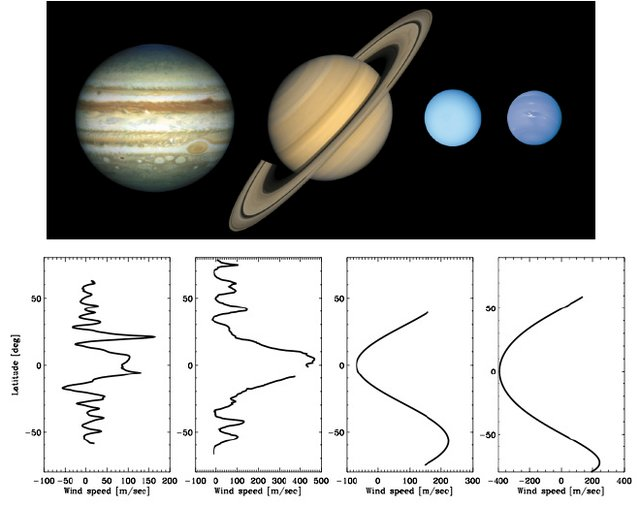
\includegraphics[clip,width=9cm]{./fig/intro/fig1.jpg}
    \caption{
      \footnotesize{上段 : 木星,土星,
天王星,海王星の可視光領域画像.
下段 : 縦軸が緯度,横軸が
クラウドトラッキングによって得られた
東西平均した東西風速分布.
巨大ガス惑星(木星,土星)は赤道域で幅の広い西風と
中緯度で東風/西風ジェットが交互に
約20個の縞状構造を形成しているのに対し,
巨大氷惑星(天王星,海王星)は
赤道域で幅の広い東風ジェットを含め
3つのジェットを形成している
\citep{showman2009atmospheric}.
      }
    }
    \label{fig1}
  \end{center}
\end{figure}
\clearpage
%
一方,極域の観測では
低中緯度ではあまり見られない空間スケールの大きい
低気圧性渦(自転と同じ向きに回転する渦)が
存在し,そのレジームが巨大惑星ごとに
異なることが近年のJuno, Cassini といった探査機の観測によって明らかになった.
%
図\ref{fig2} に木星と土星の極域観測を示した.
木星では複数の低気圧性渦が極付近にある低気圧性渦を
取り囲んでいるという特徴がある.
%
北極域では極から約$0.5^\circ$ 離れた位置に
低気圧性渦があり,その渦の周りを
8つの低気圧性渦が囲んでいる.
それぞれの渦の半径は約2000 - 2300 km (緯度幅で$\sim 2^\circ$) である.
%
南極域では極から約$1 \sim 2 ^\circ$ 離れた位置に
低気圧性渦があり,その渦の周りを
5つの低気圧性渦が囲んでいる.
それぞれの渦の半径は北極域のものより大きく,
約2800 - 3500 km (緯度幅で$\sim 3^\circ$) である\citep{Adriani2018}.

複数の低気圧性渦が存在する木星に対し,
土星では半径約2000 km (緯度幅で$\sim 2^\circ$) の
単一の低気圧性渦が各極域を支配している.
%
天王星,海王星もVoyger 2号と地上観測から
土星の低気圧性渦よりもサイズの大きい,
単一の低気圧性渦(緯度幅で$\sim 10^\circ$)が存在することが
示唆されている.
%
\begin{figure}[t]
  \begin{center}
    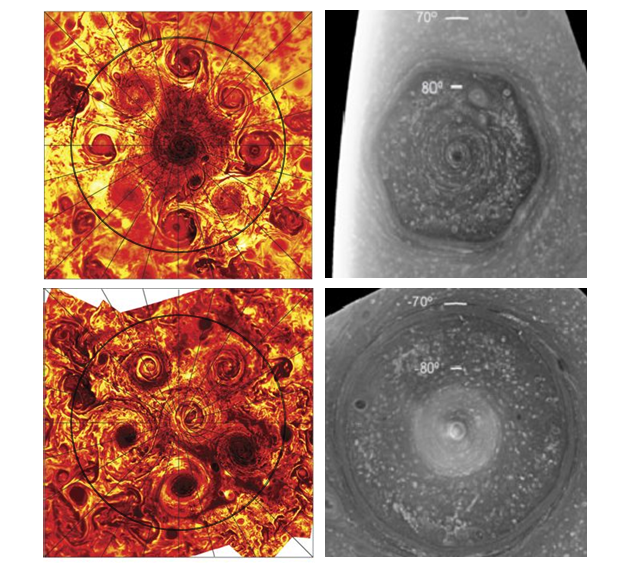
\includegraphics[clip,width=8cm]{./fig/intro/fig2.png}
    \caption{
      \footnotesize{左はJuno による木星観測(波長 : $5 \rm{\mu m}$).
黒の等緯度線は$80^\circ$ \citep{Adriani2018}.
右はCassini による土星観測(波長 : 750 nm) \citep{Antuano2015}.
上は北極域,下は南極域である.
      }
    }
    \label{fig2}
  \end{center}
\end{figure}
%
%
%\def\intro2{先行研究}
\section{先行研究}
\label{sec:intro2}
巨大惑星の内部構造の観測が難しいこともあり,
大気循環の力学的描像と理解は
数値計算を行い,\ref{sec:intro1}節で
述べた表層流の特徴の再現を通して,理解を試みてきた.
%
しかし,巨大惑星の内部構造は内部熱源があることなど,
地球型惑星の内部構造と大きく異なっており,
地球大気とのアナロジーで表層流を理解することは難しい.
特に,数値計算を行う際に問題になるのは
観測される表層の大気運動の深さである.
これについては大きく分けて,2つの説が考えられている.
%
1つは惑星内部の対流層と観測可能な雲が存在する大気上層部の
大気の運動が直接つながっているとする「深いモデル」である.
このモデルにおいては比較的,赤道域で強い西風ジェットは
形成されるものの,中高緯度域の縞状構造が発達しないという
問題点がある\citep{CHRISTENSEN2002}.
%
もう1つは,惑星深部の対流と大気上層部の対流は独立しており,
深部からの強制はあるものの深部の対流とは別のメカニズムで
構造が形作られているという「浅いモデル」である.
このモデルでは比較的,中高緯度の縞状構造が形成されるが,
赤道での西風ジェットが形成しないという問題点がある\citep{Scott2007}.
%
現在のところ決定的な議論は出来ていない.
%
\subsection{Showman et al. (2007)}
\label{sec:intro21}
これまでの「浅いモデル」の研究では
初期に小スケールの乱流を与え,時間発展をみる
自由減衰乱流実験\citep{Yoden1993}や
小規模な渦度強制を加える実験\citep{Scott2007}などが行われてきた.
%
しかし,このような全球的かつ連続的な
強制が巨大惑星に働いているとは考えにくい.
%
擾乱を引き起こす現象として
木星,土星で観測されている
雷雲(\cite{Gierasch2000}, \cite{Porco2005})が考えられている.
%
\cite{Showman2007}はこの雷雲を想定した
局所的かつ離散的な強制を与え,球面浅水実験を行った.
彼らは緯度$0 - 70^\circ$,経度$0 - 120^\circ$の範囲の領域を計算した.
その結果,中緯度の変形半径が小さい場合($< 2000$ km) には図\ref{fig3} のように
赤道域で幅の広い東風ジェットが形成し,
中緯度では渦が支配的になることがわかった.
%
中緯度の変形半径が大きい場合($> 4000$ km) には,
弱い渦は伴うものの,ジェットが支配的にな
ことがわかった.
%
雷雲の強さ,ニュートン冷却の緩和時間などの
パラメータを変更した実験を行ったが,
どのケースも赤道域では東風ジェットになり,
木星,土星で見られるような赤道加速は見られなかった.
%
\begin{figure}[H]
  \begin{center}
    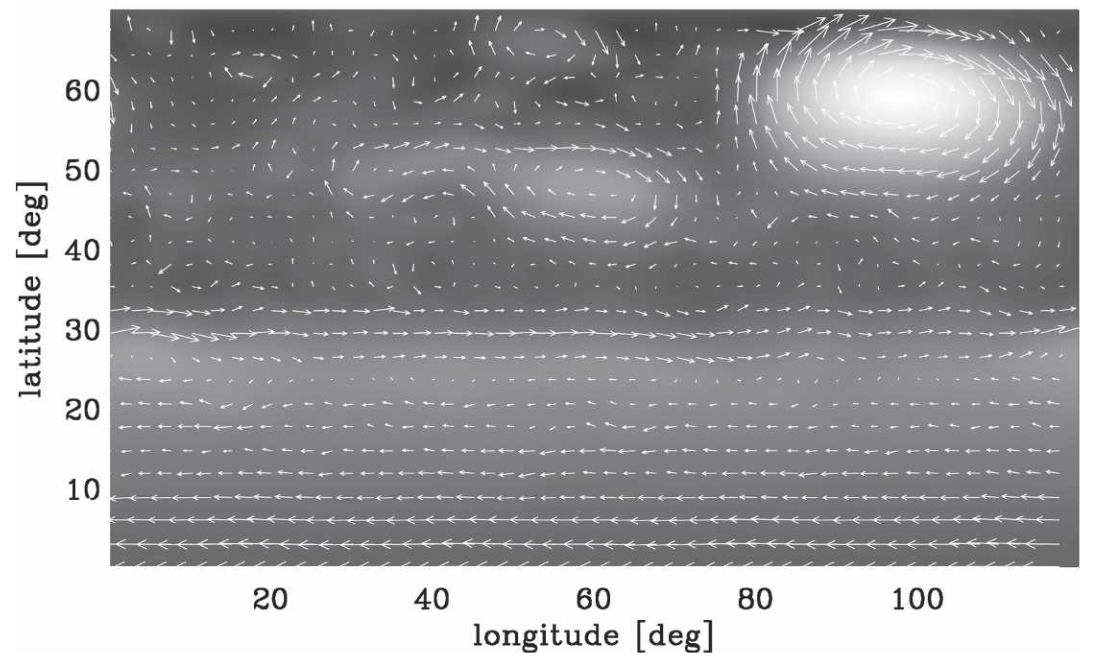
\includegraphics[clip,width=9cm]{./fig/intro/fig3.png}
    \caption{
      \footnotesize{\cite{Showman2007}のジオポテンシャルと
速度ベクトルの計算結果(4190地球日,中緯度の変形半径 : $L_d \sim 1200$ km).
      }
    }
    \label{fig3}
  \end{center}
\end{figure}
%
\subsection{Brueshaber et al. (2019)}
\label{sec:intro22}
\cite{Brueshaber2019}は\cite{Showman2007}の雷雲を
想定した強制浅水実験を極域(約$\sim 60^\circ$ の等緯度線より高緯度)で計算し,
極渦とそのレジームに注目した.
その結果,図\ref{fig4}に示すようにBurger 数 : $Bu = (L_{d0}/a)^2$ と呼ばれる
極での変形半径 : $L_{d0}$ と惑星半径 : $a$ で書かれる無次元量の値によって,
極渦のレジームが変化することがわかった.
%
Burger 数の値が$Bu \leq 2.40 \times 10^{-4}$の場合,
木星で観測されるような極のまわりを囲むような
配置は見られないが,複数の小さな低気圧性渦が形成する.
この特徴からこのレジームを木星的と分類した.
%
Burger 数の値が$4.00 \times 10^{-4 } \leq  Bu \leq  8.16 \times 10^{-4}$の場合,
高気圧性渦と低気圧性渦が混在するレジームがあらわれる.
Burger 数が木星的レジームと土星的レジームの間にあるため
このレジームを遷移状態と分類した.
%
Burger 数の値が$8.16 \times 10^{-4 } \leq Bu \leq  2.50 \times 10^{-3}$の場合,
土星で観測されるような極を中心とした単一の低気圧性渦が形成する.
この特徴からこのレジームを土星的と分類した.
%
Burger 数の値が$Bu \geq 4.44 \times 10^{-3 }$の場合,
土星的レジームよりも強力な極を中心とした単一の低気圧性渦が形成する.
この特徴からこのレジームを氷巨大惑星的と分類した.
%
\begin{figure}[H]
  \begin{center}
    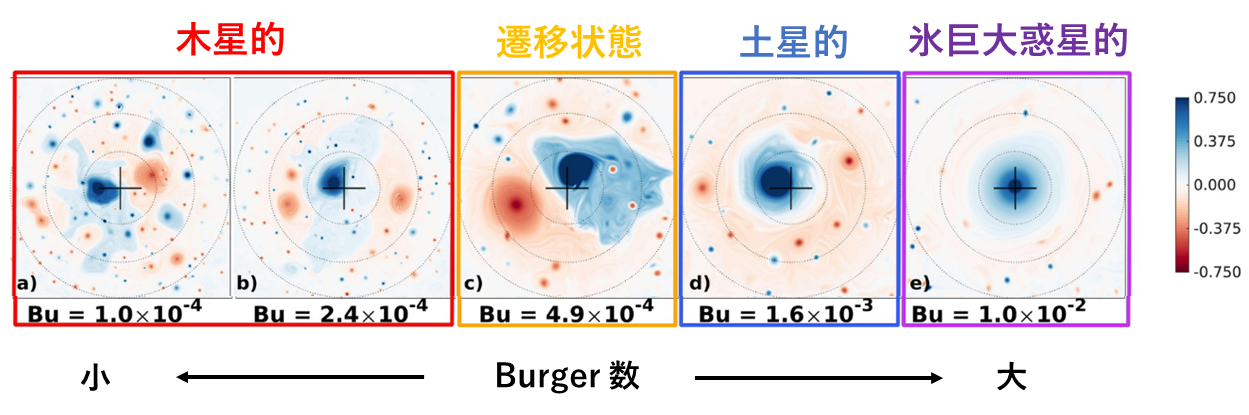
\includegraphics[clip,width=14cm]{./fig/intro/fig4_1.png}
    \caption{
      \footnotesize{\cite{Brueshaber2019}の無次元ポテンシャル渦度 : $Q_e^*$ の計算結果(20000地球日).
Burger 数の値に応じて巨大惑星で観測されるような極渦のレジームが変化する.
$Q_e^* = 0$ は静止流体(相対渦度や流体層の厚さの水平平均からの変化はない),
$Q_e^* > 0$ は低気圧性渦,$Q_e^* < 0$ は高気圧性渦を表す.
      }
    }
    \label{fig4}
  \end{center}
\end{figure}
%
\def\intro3{研究目的}
\section{\intro3}
\label{sec:intro3}
木星,土星で観測される雷雲を想定した強制を与えた浅水数値実験を
\cite{Showman2007}は低緯度から中緯度の領域を計算し,
赤道域のジェットと縞状構造に着目した.
境界条件としては,経度方向に周期境界,緯度方向はfree - slip 境界 である.
%
一方,\cite{Brueshaber2019}は極域の領域で計算を行い,
極渦のレジームに着目した.
境界条件としては,周期境界だが,スポンジ層により,流れは減衰する.
%
どちらの先行研究も領域計算であり,
このような領域の制限は流れ場全体の構造に影響を与える可能性がある.
例えば,\cite{Brueshaber2019} では低緯度からの運動量輸送が考慮できていなく,
これは,現実的ではない.
%
%
%例えば,\cite{Heimpel2007}は薄い球殻領域内の
%深部対流運動を全球の1/8 の領域で解き,
%縞状構造と赤道加速が共存する状態を数値的に再現した.
%しかし,この計算を全球で計算した
%\cite{Takehiro2015}では時間積分を進めると縞状構造が
%消滅するという結果がある.
%
そのため本研究では,雷雲を想定した
強制浅水実験を全球で行い,
低緯度から中緯度の主に東西ジェットの構造を
\cite{Showman2007}の計算と比較,
極域の渦の構造を\cite{Brueshaber2019}と比較する.
そして,雷雲を想定した強制により,
\ref{sec:intro1}節で述べた巨大惑星の表層流の特徴が
雷雲による強制により,形成されるのかを調べることが
本研究の目的である.
%
\def\intro4{本論文の構成}
\section{\intro4}
\label{sec:intro4}
本論文の構成を簡単に述べる.
\ref{chap:2}章では用いた1.5層浅水方程式系と
数値実験の手法および設定について述べる.
\ref{chap:3}章ではBurger 数,放射緩和時間,
低気圧性渦/高気圧性渦の割合,解像度のそれぞれの
値を変化させたときの実験結果を示す.
\ref{chap:4}章では
東西ジェットと極渦のレジームに注目し考察を行う.
\ref{chap:5}章で本論文の結論を述べる.
%
%
\setcounter{table}{0}
\def\chap2{モデルと手法}
\chapter{\chap2}
\label{chap:2}
\markright{2 \chap2}
ここでは本研究で用いるモデルと実験手法・実験設定について述べる.
\section{支配方程式系}
\label{sec:model1}
本研究では球面上の1.5層浅水方程式系を用いる.
これは\cite{Showman2007}, \cite{Brueshaber2019}で用いられた系と同じである.
このモデルにおいて上層と下層はそれぞれの層で密度一定であり,
上層は活動的な層,下層は無限に深く静止したそうであると仮定する.
上層に対する運動量方程式と質量保存の式は
%
\begin{align}
& \DD{\Dvect{u}}{t}+ g' \Dgrad h + f \Dvect{k} \times \Dvect{u} = -\Dvect{D}_{\Dvect{u}},  \label{eq:eq1} \\
& \DP{g'h}{t} + \Ddiv (g'h\Dvect{u}) = \Sigma S_{{\rm{storm}}} + S_{{\rm{rad}}} - D_h \label{eq:eq2} 
\end{align}
%
である\footnote{導出は付録 \ref{ape:A}を参照.}.
$\Dvect{u}$は水平風速,$g'$は有効重力加速度,
$h$は上層の厚さ,$f$はコリオリパラメータ,
$\Dvect{k}$は鉛直方向の単位ベクトル,
$\Dvect{D}_h, D_h$はそれぞれ計算が
発散しないための数値粘性・拡散項\footnote{詳細は付録\ref{ape:B}を参照.},
$S_{{\rm{storm}}}$は雷雲を想定した質量強制項,$S_{{\rm{rad}}}$ は放射緩和項である.
また,物質微分は
\begin{align}
\DD{}{t} = \DP{}{t} + \frac{u}{a\cos{\vartheta}} \DP{}{\lambda}
+\frac{v}{a} \DP{}{\vartheta}.
\end{align}
それぞれの強制項は
\begin{align}
&S_{{\rm{storm}}} = s \cdot \exp \left [- \frac{R^2}{R_{{\rm{storm}}}^2} - \frac{(t^*-t_0)^2}{\tau_{{\rm{storm}}}^2} \right ], \label{eq:eq3}\\
&S_{{\rm{rad}}}  = - \frac{\langle g'h \rangle - g'h_{{\rm{eq}}}}{\tau_{{\rm{mass}}}} - \frac{g'h - \langle g'h \rangle}{\tau_{{\rm{APE}}}} \label{eq:eq4}
\end{align}
である.
%
ここで,$s$は質量強制の最大値,
またその正負の割合を$\alpha$とする.
$\alpha=1.0$ のとき,正の質量強制のみが与えられる
(つまり,高気圧性渦が質量強制を与えた場所で発生する).
$R$は質量強制の中心位置からの距離,
$R_{{\rm{storm}}}$は質量強制の半径,
$t^*$は質量強制が局所的に与えられてからの時間,
$t_0$は質量強制がピークを迎える時間,
$\tau_{{\rm{storm}}}$は質量強制の特徴的な緩和時間,
$\langle \rangle$ はその瞬間の水平平均,
$h_{{\rm{eq}}}$は平衡状態での厚さ,
$\tau_{{\rm{mass}}}$はエネルギーに影響を与えず,
$\langle h \rangle $を$h_{{\rm{eq}}}$に向かって平衡化するときの緩和時間,
$\tau_{{\rm{APE}}}$は質量に影響を与えず,
$h$を$\langle h \rangle$に向かって平衡化するときの緩和時間である.
図\ref{fig5}に質量強制のスナップショットを示す.
%
\begin{figure}[t]
  \begin{center}
    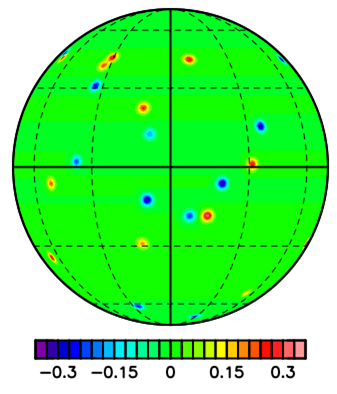
\includegraphics[clip,width=6cm]{./fig/model/fig5_v2.png}
    \caption{
      \footnotesize{質量強制 : $S_{{\rm{storm}}}$ のスナップショット($s_{max} = 0.333$, $R_{{\rm{storm}}} = 2.62 \times 10^6 {\rm{~m~}}(2.1^{\circ})$
, $\alpha = 0.5$の場合).
ある時刻と位置に雷雲を想定した質量強制を式(\ref{eq:eq3})で与える.
質量強制は$R > 2.2 R_{{\rm{storm}}}, t^* > 2.2 \tau_{{\rm{storm}}}$ で0とする.
質量強制が与えられてから,$2.2 \tau_{{\rm{storm}}}$ 秒後に消滅.
そこから$\tau_{interval}$ 秒後に違う位置に質量強制が与えられる.
      }
    }
    \label{fig5}
  \end{center}
\end{figure}
%
質量強制は$R > 2.2 R_{{\rm{storm}}}, t^* > 2.2 \tau_{{\rm{storm}}}$ で0 とする.
質量強制が与えられてから,$2.2 \tau_{{\rm{storm}}}$ 秒が経過し,消滅後,
そこから$\tau_{interval}$ 秒後に違う位置に質量強制が与えられる.

式(\ref{eq:eq4}) の放射緩和項の右辺第1項は
緩和時間$\tau_{{\rm{mass}}}$ で$\langle h \rangle $を
平衡厚さ$h_{{\rm{eq}}}$に向かって,緩和する.
%
右辺第2項は緩和時間$\tau_{{\rm{APE}}}$ で
局所的な流体層の厚さの変化を$\langle h \rangle $に向かって,緩和する.
%
これら2つの項により,統計的定常状態を実現する.
%
\cite{Brueshaber2019} ではこれらの強制項に加え,加えた質量強制を層から差し引く
質量調整項を加えていたが,ここでは\cite{Showman2007}にならい,加えない.使用する記号を表\ref{table:para}にまとめる.
\begin{table}[t]
  \caption{本論文中で使用する記号一覧}
  \label{table:para}
  \begin{center}
    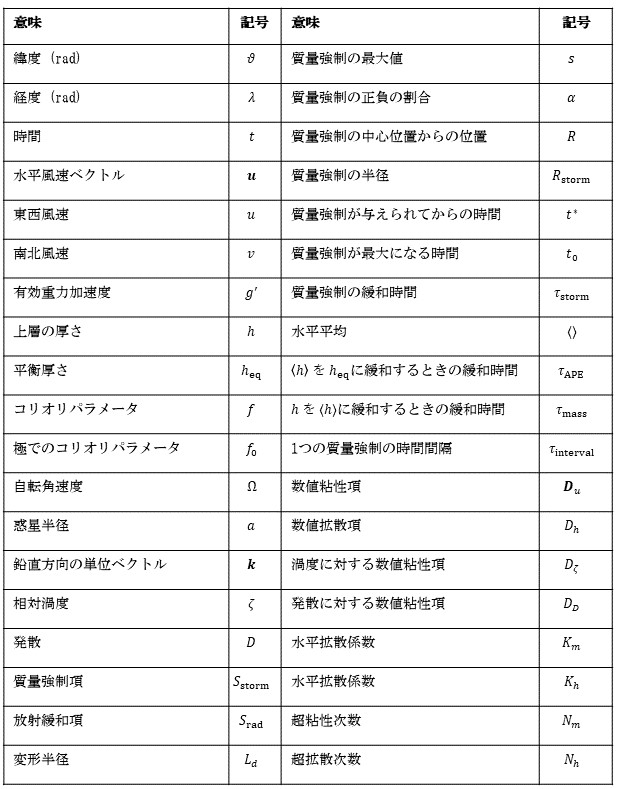
\includegraphics[clip,width=15cm]{./fig/model/table_para-2.jpg}
  \end{center}
\end{table}
%
\clearpage
\newpage
\section{実験手法・実験設定}
\label{sec:model2}
球面上の支配方程式系(\ref{eq:eq1}), (\ref{eq:eq2}) を解く.
その際,運動量方程式はベクトル量である速度のままだと
球面座標系では格子点が集中する極点付近で,計算が難しい.
そのため,式(\ref{eq:eq1})を変形しスカラー量である渦度と発散に関する式を用いる\footnote{付録 \ref{ape:B} を参照.}.
%
また,数値的な安定性を維持するために
ラプラシアン4次の超粘性を加える.
%
空間離散化にはスペクトル法を用いる.
時間離散化は数値粘性項についてはクランク・ニコルソン法,
それ以外の項には4次のルンゲクッタ法を用いる.
%
また数値モデルの作成には地球流体電脳倶楽部の階層的地球スペクトルモデル集
(SPMODEL; \cite{spmodel2006}, \cite{spmodel2013}) を使用する.
%
初期に上層は静止しており,$10 \tau_{interval}$ 秒経過する間に
最初の質量強制がランダムな位置に最大で50個加えられる.
%
自転角速度は木星の値を用いる.
また,計算時間は3000 地球日とする.
%
本研究で用いた共通パラメータを表\ref{table1} に示す.
表\ref{table2}に計算を行った数値実験のケースとその用いたパラメータを示す.

以下ではA1 のケースを標準実験とし,\ref{sec:A1}節でその実験結果について述べる.
%
その次に,\ref{sec:case1}節では$g'h_{{\rm{eq}}}$の値を変化させ,Burger 数の影響を調べた実験1の結果について示す.
\ref{sec:case2}節では$\tau_{{\rm{APE}}}$の値を変化させ,放射緩和の影響を調べた実験2の結果について示す.
\ref{sec:case3}節では$\alpha$の値を変化させ,質量強制の正負の影響を調べた実験3の結果について示す.
\ref{sec:case4}節では解像度の違いによる変化を調べた実験4の結果について示す.
\begin{table}[ht]
  \caption{実験で用いた共通パラメータ}
  \label{table1}
  \begin{center}
    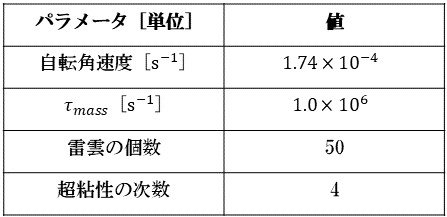
\includegraphics[clip,width=8cm]{./fig/model/table1.jpg}
  \end{center}
\end{table}
%
\newpage
\begin{landscape}
\begin{table}[t]
  \caption{実験のケースと用いたパラメータ}
  \label{table2}
  \begin{center}
    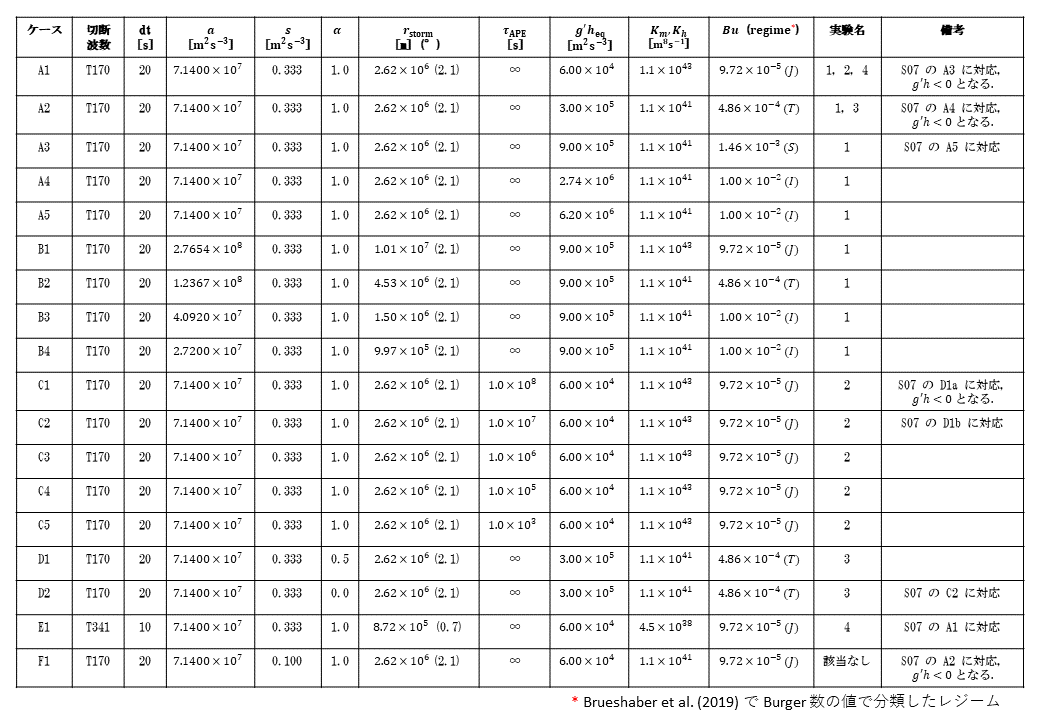
\includegraphics[clip,width=20cm]{./fig/model/table2_v2.png}
  \end{center}
\end{table}
\end{landscape}
%
\clearpage

\def\chap3{実験結果}
\chapter{\chap3}
\label{chap:3}
\markright{3 \chap3}
%
\section{標準実験結果 : A1}
\label{sec:A1}
ここでは,標準実験とした A1 のケースの結果を図\ref{fig:A1_1}-\ref{fig:A1_5}に示す.
用いたパラメータは表\ref{table2}を参照.
図\ref{fig:A1_1}の東西風速を見てわかるように,
赤道域で幅が広く,風速が約$220 \rm{~m \cdot s^{-1}}$と強力な東風ジェットと
緯度約$\pm 30^\circ$ で風速約$100 \rm{~m \cdot s^{-1}}$の西風ジェットが見られる.
%
また,その西風ジェットに対応して,図\ref{fig:A1_2}のジオポテンシャルが
その領域で値が小さくなっている.
%
正(負)の質量強制の場合,流体層に局所的な膨らみ(窪み)を作る.
この局所的に膨らんだ場所はコリオリ力により,高気圧性(低気圧性)渦を形成する.
%
このケースでは正の質量強制のみ与えられるため,
図\ref{fig:A1_3}の相対渦度分布を見て分かるように,
高気圧性渦が見て取れる.
さらに,渦の正負を分かりやすくするために,無次元ポテンシャル渦度を定義する.
%
無次元ポテンシャル渦度 : $Q_e^*$は
\begin{align}
Q_e^* = \left [\frac{\zeta+f}{h}-\frac{f}{\langle h \rangle}\right]\cdot \frac{\langle h \rangle}{f_0}
\end{align}
である.ここで,$\zeta$は相対渦度,$f$はコリオリパラメータ,$f_0$は極でのコリオリパラメータの値である.
%
$Q_e^*=0$は静止流体(相対的な渦度や厚さの摂動はない)を表す.
$Q_e^*>0$は低気圧性の渦度を表し,
$Q_e^*<0$は高気圧性の渦度を表す.
%
図\ref{fig:A1_4}の極域を見てみると巨大な低気圧性渦の中に,複数の高気圧性渦が形成していることがわかる.
%
図\ref{fig:A1_5}に有効ポテンシャルエネルギー : APE と運動エネルギー : KE 
\begin{align}
APE &= \frac{1}{2} \int \left[(g'h)^2 - \langle g'h \rangle^2   \right] dA. \\
KE  &= \frac{1}{2} \int g'h(u^2 + v^2) dA.
\end{align}
を示す.ここで,$A$ は計算領域の面積,$u, v$ はそれぞれ経度,緯度方向の速度である.
%
A1 のケースでは$\tau_{{\rm{APE}}} = \infty$ のため,APE とKE は時間とともに増加する.
\begin{figure}[b]
  \begin{center}
    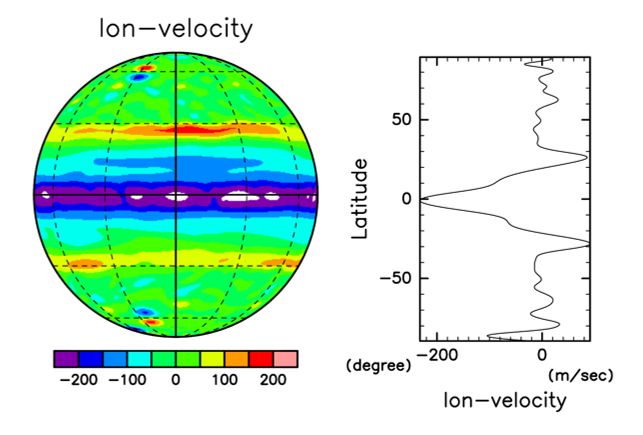
\includegraphics[clip,width=10cm]{./fig/result/A1/A1_1.png}
    \caption{
      \footnotesize{A1の実験結果. 左 : 東西風速,右 : 東西平均した東西風速(3000 地球日).
      }
    }
    \label{fig:A1_1}
  \end{center}
\end{figure}
%
\begin{figure}[ht]
  \begin{center}
    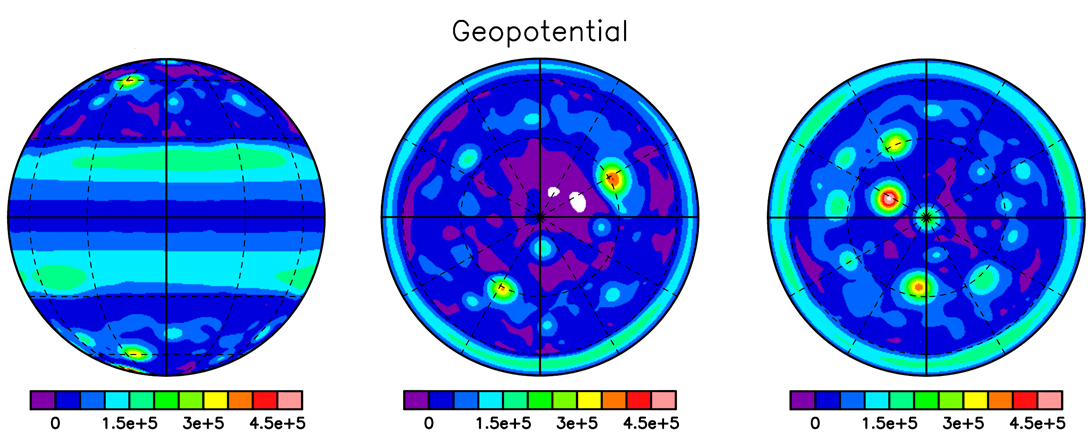
\includegraphics[clip,width=12cm]{./fig/result/A1/A1_2.png}
    \caption{
      \footnotesize{A1の実験結果. ジオポテンシャル(3000 地球日).
左 : 緯度$0^\circ$,経度$0^\circ$から見た球面投影.
中 : 緯度$90^\circ$,経度$0^\circ$から見た球面投影.
右 : 緯度$-90^\circ$,経度$0^\circ$から見た球面投影.
      }
    }
    \label{fig:A1_2}
  \end{center}
\end{figure}
%
\begin{figure}[ht]
  \begin{center}
    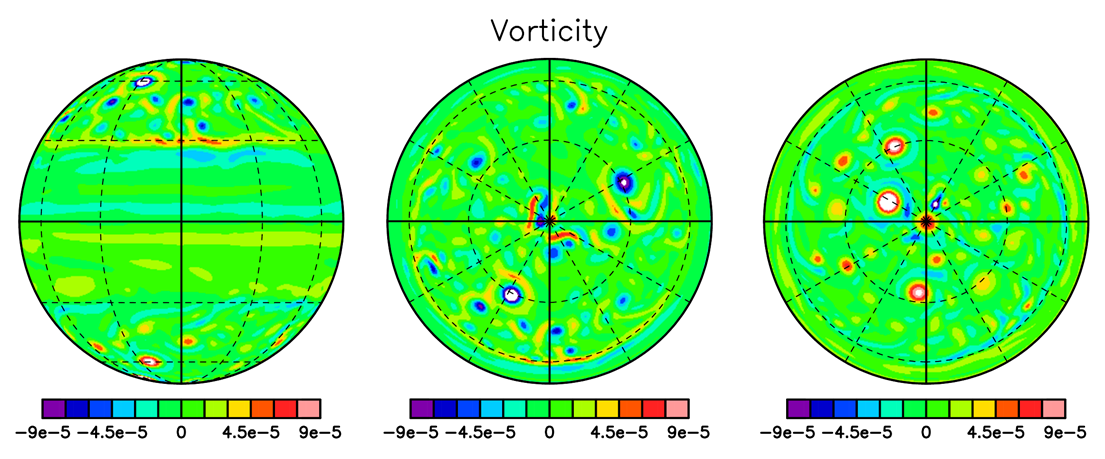
\includegraphics[clip,width=12cm]{./fig/result/A1/A1_3.png}
    \caption{
      \footnotesize{A1の実験結果. 相対渦度(3000 地球日).
左 : 緯度$0^\circ$,経度$0^\circ$から見た球面投影.
中 : 緯度$90^\circ$,経度$0^\circ$から見た球面投影.
右 : 緯度$-90^\circ$,経度$0^\circ$から見た球面投影.
      }
    }
    \label{fig:A1_3}
  \end{center}
\end{figure}
%
\begin{figure}[ht]
  \begin{center}
    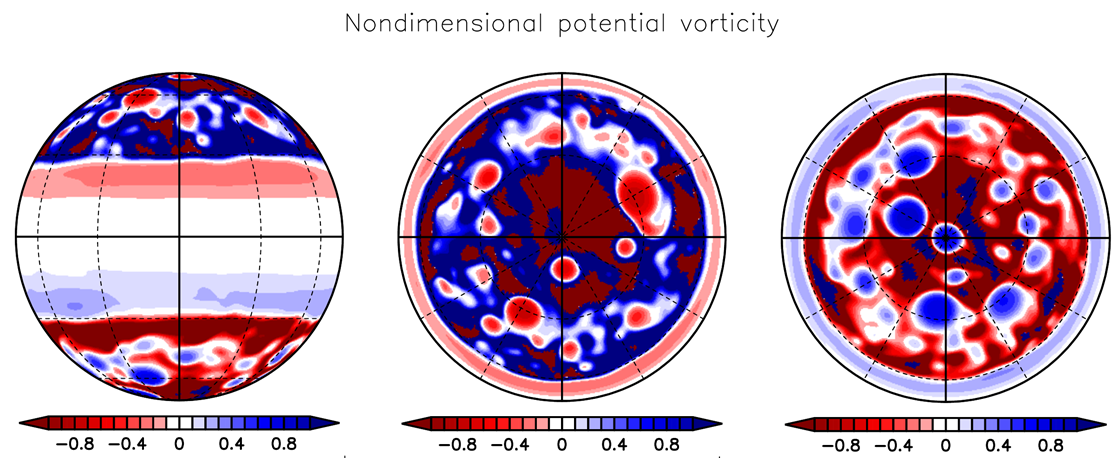
\includegraphics[clip,width=12cm]{./fig/result/A1/A1_4.png}
    \caption{
      \footnotesize{A1の実験結果. 無次元ポテンシャル渦度(3000 地球日).
左 : 緯度$0^\circ$,経度$0^\circ$から見た球面投影.
中 : 緯度$90^\circ$,経度$0^\circ$から見た球面投影.
右 : 緯度$-90^\circ$,経度$0^\circ$から見た球面投影.
      }
    }
    \label{fig:A1_4}
  \end{center}
\end{figure}
%
\begin{figure}[ht]
  \begin{center}
    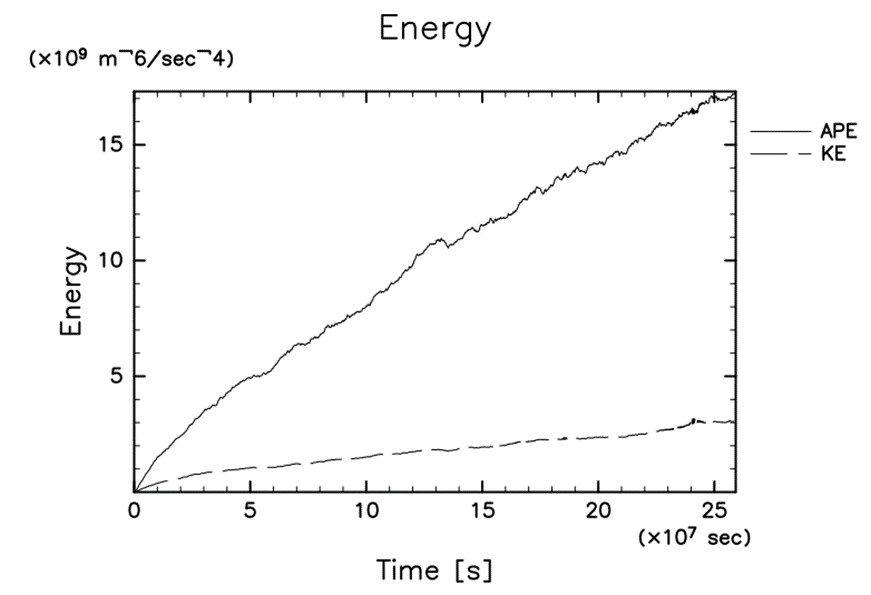
\includegraphics[clip,width=12cm]{./fig/result/A1/A1_5.jpg}
    \caption{
      \footnotesize{A1の実験結果. 有効ポテンシャルエネルギー : APE (実線) と運動エネルギー : KE (点線) の時間発展.
      }
    }
    \label{fig:A1_5}
  \end{center}
\end{figure}
%
\clearpage
\newpage
\section{実験1 : Burger 数の変化による影響}
\label{sec:case1}
この節ではBurger 数 
\begin{align}
Bu = \left (\frac{L_{d0}}{a} \right )^2
\end{align}
の変化による影響を調べる.
$a$は惑星半径,$L_{d0}$は極での変形半径
\begin{align}
L_{d0} = \frac{\sqrt{g'h_{{\rm{eq}}}}}{f_0}, \qquad f_0 = 2 \Omega
\end{align}
である.\cite{Brueshaber2019}ではBurger 数を初期の値から
変化しないように,質量強制によって加えられた質量を
全球の流体層の厚さから取り除く項を入れているが,
本研究では平衡厚さ$g'h_{{\rm{eq}}}$でBurger 数を定義する.
図\ref{fig:case1_1}にBurger 数を変化させて行った実験の
無次元ポテンシャル渦度を示す.
図の下に示されているアルファベットは\cite{Brueshaber2019}が
Burger 数によって,分類した極渦のレジームを示している.
それぞれ,次の特徴によって,分類されている.
\begin{itemize}
  \item J - 木星的レジーム
  \begin{itemize}
   \item 複数の渦が発生し,極に渦がとどまらない.
  \end{itemize}
  \item T - 遷移的レジーム
  \item S - 土星的レジーム
  \item I - 巨大氷惑星的レジーム
\end{itemize}
%
\begin{figure}[ht]
  \begin{center}
    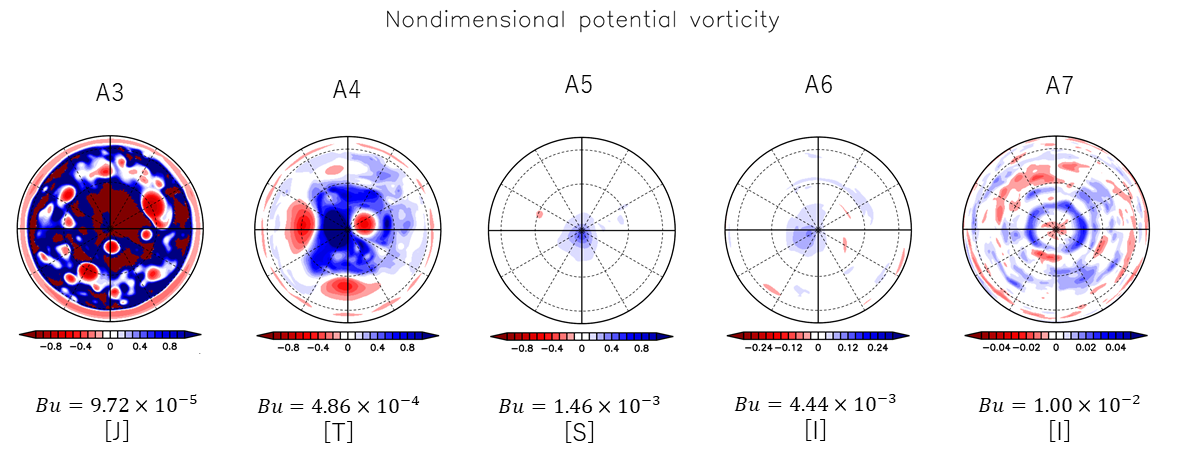
\includegraphics[clip,width=14cm]{./fig/result/case1/case1_1.png}
    \caption{
      \footnotesize{無次元ポテンシャル渦度(3000 地球日).
上にケース,下にBurger 数と\cite{Brueshaber2019}で分類された極渦のレジームを示している.
      }
    }
    \label{fig:case1_1}
  \end{center}
\end{figure}
%
\begin{figure}[ht]
  \begin{center}
    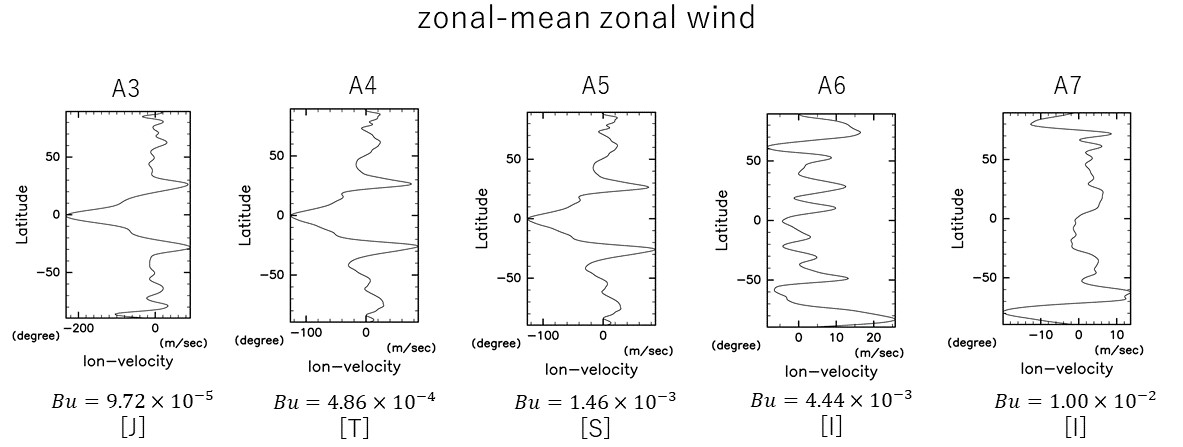
\includegraphics[clip,width=14cm]{./fig/result/case1/case1_2.jpg}
    \caption{
      \footnotesize{東西平均した東西風速(3000 地球日).
上にケース,下にBurger 数と\cite{Brueshaber2019}で分類された極渦のレジームを示している.
      }
    }
    \label{fig:case1_2}
  \end{center}
\end{figure}

\def\chap4{考察}
\chapter{\chap4}
\label{chap:4}
\markright{4 \chap4}
ddd

\def\chap5{結論}
\chapter{\chap5}
\label{chap:5}
\markright{5 \chap5}
sss



%%% Appendix %%%
%%%%%%%%%%%%%%%%
%\setcounter{chapter}{1} % chapter の番号をゼロにリセットする
%\setcounter{section}{0} % section の番号をゼロにリセットする
\stepcounter{chapcounter}
\stepcounter{seccounter}

\renewcommand{\thesection}{\Alph{section}} % 数字ではなくアルファベットで数える

def\thesection{\Alph{section}}
\def\theequation{\Alph{section}.\arabic{equation}}

\chapter*{付録}
\addcontentsline{toc}{chapter}{付録}
%%  A  %%
\def\apetitleA{: 1.5層浅水方程式系の導出}
\def\apeA{\Alph{section} \apetitleA}
\section{\apetitleA}
\label{ape:A}
\markright{\apeA}
%% Appendix A %%
%%%%%%%%%%%%%%%%
\setcounter{subsection}{0}
\setcounter{subsubsection}{0}
\setcounter{figure}{0}
\setcounter{table}{0}
\setcounter{equation}{0}
\renewcommand{\thesubsection}{\Alph{section}.\arabic{subsection}} 
\renewcommand{\thesubsubsection}{\Alph{section}.\arabic{subsection}.\arabic{subsubsection}} 
\renewcommand{\thefigure}{\Alph{section}.\arabic{figure}}
\renewcommand{\thetable}{\Alph{section}.\arabic{table}}
%
$B$3$3$G$O!$(B\cite{Vallis2017} 3.2$B@a(B $BM-8z=ENO$NJ}Dx<07O$r;29M$K!$(B
1.5$BAX@u?e%b%G%k$NJ}Dx<0$rF3=P$9$k!%(B
\subsection*{$B!&(B1.5 $BAX@u?e%b%G%k$N35MW(B}
$B@u?e7O$G:G$bC1=c$J(B1$BAX%b%G%k$O(B
$BL)EY$,JQ2=$7$J$$0lAX$NN.BNAX$r9M$($F$$$k!%(B
%
%
\begin{figure}[b]
 \begin{center}
 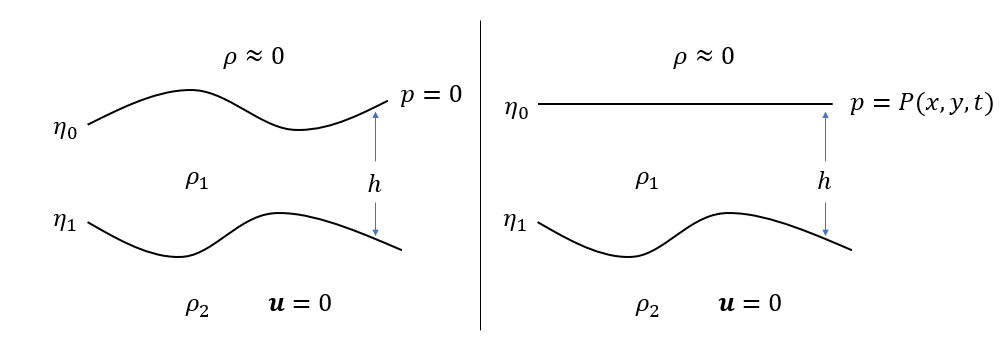
\includegraphics[clip,width=13cm]{./appendix/A/fig/one-half-fig1.png}
 \end{center}
 \caption{1.5$BAX@u?eJ}Dx<07O$NLO<0?^!!(B(\cite{Vallis2017} $B$N?^(B3.3 $B$r2~JQ(B).
$B:8$O<+M3I=LL6a;w!$1&$O9dBNI=LL6a;w$G$"$k!%(B
$B>eAX$N8|$5(B$h$$B$O>eAX$N9b$5(B$\eta_0$$B$H2<AX$N9b$5(B$\eta_1$$B$rMQ$$$F!$(B
$h=\eta_0 - \eta_1$$B$G=q$+$l$k!%(B
} 
 \label{figA1}
\end{figure}
%
$B$7$+$7!$8=<B$NN.BN$NL)EY$OJQ2=$9$k$O$:$G$"$k!%(B
$BFC$K@.AX$7$F$$$l$P!$1tD>J}8~$KJQ2=$9$k$H9M$($i$l$k!%(B
1.5$BAX%b%G%k$G$O>eAX$O3hF0E*!$(B
$B2<AX$OL58B$K?<$/@E;_$7$?L)EY$N0[$J$k(B2$B$D$NN.BNAX$r9M$(!$(B
$BC1=c$G$O$"$k$,1tD>J}8~$NL)EYJQ2=$r9MN8$9$k!%(B
%
$B3$MN$G$O2<AX$O$[$H$s$I@E;_$7!$(B
$B1?F0$N$"$k>eAX$O?t(B100 m $B$N8|$5$G$"$k$?$a!$(B
$B$3$N%b%G%k$,;H$o$l$k$3$H$,$"$k!%(B
%
$B?^(B\ref{figA1}$B$K(B1.5$BAX%b%G%k$NLO<0?^$r<($9!%(B
$B$3$3$G!$(B$\eta_0$$B$O>eAX$N9b$5!$(B
$\eta_1$$B$O2<AX$N9b$5!$(B$h$$B$O>eAX$N8|$5!$(B
$B>eAX!$2<AX$NL)EY$O$=$l$>$l(B$\rho_1, \rho_2~(\rho_1 < \rho_2)$ $B$G$"$k!%(B
$B>eC<$N6-3&>r7o$O<+M3I=LL$H9dBNI=LL$N(B2$B$D$N>l9g$,$"$k!%(B
\cite{Showman2007}, \cite{Brueshaber2019} $B$G$O(B
$B9dBNI=LL6a;w$rMQ$$$F$$$k$H9M$($i$l$k!%(B
$B0J2<$G$O$=$l$>$l$N6-3&>r7o$N>l9g$GJ}Dx<07O$rF3$/!%(B
%
%\cite{Showman2007} $B$G$O(B
%$B>eAX$O@ENO3XE*$K0BDj$7$?BPN.7w>eIt(B (5 - 10 bar $B$N(B
%$B?e$N6E7k%l%Y%kIU6a$+$i>e$NAX$N8|$5(B)$B!$(B
%$B2<AX$OL58B$K?<$/CfN)E*$K@.AX2=$7$?AX$r(B
%$B9M$($k$H5-:\$7$F$$$k!%(B
%
\subsection*{$B!&<+M3I=LL6a;w(B}
\subsubsection*{$B1?F0NLJ}Dx<0(B}
$B$^$:$O>eAX$K$D$$$F9M$($k!%>eAX$N@E?e05$N<0$O(B
\begin{equation}
\frac{\partial p_1}{\partial z}=-\rho_1 g. \label{eq:A1}
\end{equation}
$B$3$l$r!$>eAX$N>eC<(B$\eta_0$ $B$+$i$"$k?<$5(B$z$ $B$^$G@QJ,$9$k$H(B
\begin{equation}
\int_0^{p_1} dp= -\rho_1 g  \int_{\eta_0}^z dz. \label{eq:A2}
\end{equation}
$B<+M3I=LL6a;w$G$O>eAX$N>eC<$G(B$p(\eta_0) = 0$$B$J$N$G!$(B
\begin{equation}
p_1 (x, y, z, t) = \rho_1 g  (\eta_0 - z). \label{eq:A3}
\end{equation}
$B<0(B(\ref{eq:A3})$B$N?eJ?8{G[$r$H$k$H!$(B
\begin{align}
\nabla_z p_1 &= \rho_1 g \nabla_z \eta_0, \notag \\
\frac{1}{\rho_1} \nabla_z p_1 &=  g \nabla_z \eta_0. \label{eq:A4}
\end{align}
$B$3$3$G!$(B
\begin{align}
\nabla_z&=\left(\frac{\partial}{\partial x},\frac{\partial}{\partial y}\right). \notag
\end{align}
%

$B<!$K2<AX$K$D$$$F9M$($k!%(B
$B2<AX$N@E?e05$N<0$O(B
\begin{equation}
\frac{\partial p_2}{\partial z}=-\rho_2 g. \label{eq:A5}
\end{equation}
$B$3$l$r!$2<AX$N>eC<(B$\eta_1$ $B$+$i$"$k?<$5(B$z$ $B$^$G@QJ,$9$k$H(B
\begin{align}
\int_{p_1}^{p_2} dp= -\rho_2 g  \int_{\eta_1}^z dz, \notag \\
p_2 - p_1 = \rho_2 g  (\eta_1 -  z). \label{eq:A6}
\end{align}
$p_1$ $B$O<0(B(\ref{eq:A3})$B$G(B $z=\eta_1$$B$H$7$?CM$J$N$G(B
\begin{align}
p_2  &= p_1  + \rho_2 g  (\eta_1  - z) \notag \\
     &= \rho_1 g (\eta_0 - \eta_1) + \rho_2 g  (\eta_1  - z) \notag \\
     &= \rho_1 g (\eta_0 - \eta_1) + \rho_2 g  (\eta_1  - z).  \label{eq:A7}
\end{align}
%
$B<0(B(\ref{eq:A7})$B$N?eJ?8{G[$r$H$k$H!$(B
\begin{align}
\nabla_z p_2 &= \rho_1 g  (\nabla_z \eta_0 - \nabla_z \eta_1) + \rho_2 g  \nabla_z \eta_1   \notag \\
& = \rho_1 g \nabla_z \eta_0 +  \rho_1 g \frac{(\rho_2 - \rho_1)}{ \rho_1 }  \nabla_z \eta_1 \notag \\
& = \rho_1 g \nabla_z \eta_0 +  \rho_1 g'  \nabla_z \eta_1. \label{eq:A8} 
\end{align}
$B$3$3$G!$(B$g'$ $B$ODc8:=ENO2CB.EY(B(reduced gravity) 
\begin{align}
g' = g \frac{(\rho_2 -\rho_1)}{\rho_1}  \notag 
\end{align}
$B$G$"$k!%2<AX$O1?F0$,$J$$$N$G!$<0(B(\ref{eq:A8}) $B$N(B
$B:8JU$N05NO8{G[(B$\nabla_z p_2 $$B$O(B 0$B$K$J$k!%(B
$B$h$C$F!$(B
\begin{align}
 g \nabla_z \eta_0 = -  g'  \nabla_z \eta_1 . \label{eq:A9}
\end{align}
$B<0(B(\ref{eq:A4}) $B$h$j(B
\begin{align}
 \frac{1}{\rho_1} \nabla_z p_1  = -  g'  \nabla_z \eta_1 . \label{eq:A10}
\end{align}
%
$B>eAX$N2sE>$N8z2L$r4^$`HsG4@-N.BN$N1?F0NLJ}Dx<0$O(B
\begin{equation}
%\DP{\Dvect{u_1}}{t}+(\Dvect{u_1} \cdot \nabla)\Dvect{u_1}=
%-f\Dvect{k}\times \Dvect{u_1}-\frac{1}{\rho_1}\nabla_z p_1. \label{eq:A11}
\DD{\Dvect{u_1}}{t} + \frac{1}{\rho_1}\nabla_z p_1 + f\Dvect{k}\times \Dvect{u_1} = 0. \label{eq:A11}
\end{equation}
$B$3$3$G!$(B$\Dvect{k}$$B$O(B$z$$BJ}8~$NC10L%Y%/%H%k$G$"$k!%(B
$B<0(B(\ref{eq:A11})$B$K<0(B(\ref{eq:A10})$B$rBeF~$9$k$H(B
\begin{equation}
\DD{\Dvect{u_1}}{t}  - g' \nabla_z\eta_1 + f\Dvect{k}\times \Dvect{u_1} = 0 \label{eq:A12}
\end{equation}
$B$H$J$k!%(B
%
\subsubsection*{$BO"B3$N<0(B}
$BO"B3$N<0$O(B1$BAX$N@u?e7O$HF1MM$K9M$($k$3$H$,$G$-!$(B
\begin{equation}
\DP{g'h}{t}+\nabla_z (g'h\Dvect{u_1})=0$B!%(B\label{eq:A13}
\end{equation}
$B$^$H$a$k$H(B
\begin{itembox}[l]{$B<+M3I=LL6a;w(B}
\begin{align}
&\text{$B!&1?F0NLJ}Dx<0(B}$B!!(B\quad \DD{\Dvect{u_1}}{t}  - g'\nabla_z\eta_1 + f\Dvect{k}\times \Dvect{u_1} = 0
$B!!(B\tag{A.11} \\
&\text{$B!&O"B3$N<0(B}$B!!(B\qquad \DP{g'h}{t}+\nabla_z (g'h\Dvect{u_1})=0 \tag{A.12}$B!%(B
\end{align}
\end{itembox}
%
\subsection*{$B!&9dBNI=LL6a;w(B}
$BI=LL$G$N1?F0$,>.$5$$$J$i$P!$9dBNI=LL$rCV$$$?$H$$$&6a;w$r$7$F$b$h$$$@$m$&!%(B
$B>eC<$K$U$?$r$9$k$3$H$G!$>eC<$N>e2<1?F0$O5v$5$l$J$/$J$k!%(B
$B$=$N05NO$N6/@)$r(B$P(x, y, t)$$B$H$9$k!%(B
$B$^$?!$>eAX$N>eC<$r4p=`LL$K$H$j!$$=$3$G(B$z=0$$B$H$9$k(B ($\eta_0 = 0$)$B!%(B
$B<+M3I=LL6a;w$HF1MM$K>eAX$G$N@E?e05$N<0$r(B$z=0$$B$+$i$"$k?<$5(B$z$$B$^$G@QJ,$9$k$H(B
\begin{align}
\int_P^{p_1} dp= -\rho_1 g  \int_{0}^z dz, \notag \\
p_1 - P   = - \rho_1 g z. \label{eq:A14}
\end{align}
$B<0(B(\ref{eq:A14})$B$N?eJ?8{G[$r$H$k$H!$(B
\begin{align}
\nabla_z p_1 &= \nabla_z P. \label{eq:A15}
\end{align}
$B2<AX$N@E?e05$N<0$r(B$\eta_1$$B$+$i$"$k?<$5(B$z$$B$^$G@QJ,$9$k$H(B
\begin{align}
\int_{p_1}^{p_2} dp &= -\rho_2 g  \int_{\eta_1}^z dz, \notag \\
p_2 - p_1 &= \rho_2 g (\eta_1 - z), \notag \\
p_2 &= p_1 + \rho_2 g (\eta_1 - z). \label{eq:A16}
\end{align}
$p_1$ $B$K<0(B(\ref{eq:A14})$B$G(B$ z=\eta_1$ $B$K$7$?$b$N$rBeF~$9$l$P(B
\begin{align}
p_2 & = -\rho_1 g \eta_1 + \rho_2 g (\eta_1 - z) + P$B!!(B\notag \\
& = \rho_1 g h - \rho_2 g (h - z) + P. \label{eq:A17}
\end{align}
$B?eJ?8{G[$r$H$k$H(B
\begin{align}
\nabla_z p_2 & = - g (\rho_2 - \rho_1) \nabla_z h  + \nabla_z P, \notag \\
& = - \rho_1 g' \nabla_z h  + \nabla_z P . \label{eq:A18}
\end{align}
$B2<AX$G$O1?F0$,$J$$$N$G(B$\nabla_z p_2 = 0$$B!%$h$C$F(B
\begin{align}
\frac{1}{\rho_1 } \nabla_z P =   g' \nabla_z h. \label{eq:A19}
\end{align}
$B<0(B(\ref{eq:A15})$B$h$j(B
\begin{align}
\frac{1}{\rho_1} \nabla_z p_1 =  g' \nabla_z h. \label{eq:A20}
\end{align}
$B<0(B(\ref{eq:A11})$B$K<0(B(\ref{eq:A20})$B$rBeF~$9$k$H(B
\begin{equation}
\DD{\Dvect{u_1}}{t} + g' \nabla_z h + f\Dvect{k}\times \Dvect{u_1} = 0 \label{eq:A21}
\end{equation}
$B$H$J$k!%(B
%
$B$^$H$a$k$H(B
\begin{itembox}[l]{$B9dBNI=LL6a;w(B}
\begin{align}
&\text{$B!&1?F0NLJ}Dx<0(B}$B!!(B\quad \DD{\Dvect{u_1}}{t} + g'\nabla_z h
 + f\Dvect{k}\times \Dvect{u_1}  =0
$B!!(B\tag{A.21}\\
&\text{$B!&O"B3$N<0(B}$B!!(B\qquad \DP{g'h}{t}+\nabla_z (g'h\Dvect{u_1})=0 \tag{A.12}$B!%(B
\end{align}
\end{itembox}
%
$B9dBNI=LL6a;w$NJ}Dx<07O$O(B
1$BAX%b%G%k$NDlLLCO7A$,$J$$>l9g$N(B
$BJ}Dx<07O$N=ENO2CB.EY(B : $g$ $B$,Dc8:=ENO2CB.EY(B : $g'$ $B$KCV$-$+$o$k$@$1$G$"$k!%(B
%
$BK\8&5f$O$3$N9dBNI=LL6a;w$rMQ$$$k!%(B

%
\newpage
%
%%  B  %%
\def\apetitleB{: モデルで使用した方程式系}
\def\apeB{\Alph{section} \apetitleB}
\section{\apetitleB}
\label{ape:B}
\markright{\apeB}
%% Appendix B %%
%%%%%%%%%%%%%%%%
\setcounter{subsection}{0}
\setcounter{subsubsection}{0}
\setcounter{figure}{0}
\setcounter{table}{0}
\setcounter{equation}{0}
\renewcommand{\thesubsection}{\Alph{section}.\arabic{subsection}} 
\renewcommand{\thesubsubsection}{\Alph{section}.\arabic{subsection}.\arabic{subsubsection}} 
\renewcommand{\thefigure}{\Alph{section}.\arabic{figure}}
\renewcommand{\thetable}{\Alph{section}.\arabic{table}}
%
$B$3$3$G$O<B:]$K%b%G%kFb$G7W;;$7$?J}Dx<07O$r<($9!%(B
\subsection*{$B!&12EY!&H/;67?$N1?F0NLJ}Dx<0$X$NJQ7A(B}
$B1?F0NLJ}Dx<0(B(\ref{eq:eq1}) $B$O%*%$%i!<7A<0$G=q$/$H(B
\begin{align}
\DP{\Dvect{u}}{t} + (\Dvect{u}\cdot \nabla)\Dvect{u} +  g' \Dgrad h + f \Dvect{k} \times \Dvect{u} = -\Dvect{D}_{\Dvect{u}},  \label{ape:B1}
\end{align}
$B$3$3$G!$:8JUBh(B2$B9`$N0\N.9`$NItJ,$rJQ7A$9$k$H(B
\begin{align}
(\Dvect{u}\cdot \nabla)\Dvect{u} = \nabla \left ( \frac{\Dvect{u}\cdot \Dvect{u}}{2} \right) +\zeta \Dvect{k}\times \Dvect{u} \label{ape:B2}
\end{align}
$B$H$J$k!%$3$l$r<0(B(\ref{ape:B1})$B$KBeF~$9$k$H(B
\begin{align}
& \DP{\Dvect{u}}{t} +  \nabla \left ( \frac{\Dvect{u}\cdot \Dvect{u}}{2} \right) +\zeta \Dvect{k}\times \Dvect{u} +  g' \Dgrad h + f \Dvect{k} \times \Dvect{u} = -\Dvect{D}_{\Dvect{u}},  \notag \\
& \DP{\Dvect{u}}{t} +  \nabla \left ( \frac{\Dvect{u}\cdot \Dvect{u}}{2}  +  g' \Dgrad h \right) +
 (\zeta + f ) \Dvect{k}\times \Dvect{u}   = -\Dvect{D}_{\Dvect{u}} \label{ape:B3}
\end{align}
$B$H$J$k!%(B
$B<0(B(\ref{ape:B3})$B$N2sE>$HH/;6$r$H$k$H!$$=$l$>$l(B
\begin{align}
\DP{\zeta}{t}&=-\Ddiv (\zeta+f)\Dvect{u} - D_\zeta ,\label{ape:B4} \\
\DP{D}{t}&=\Dvect{k}\cdot \Drot (\zeta+f)\Dvect{u} 
-\nabla^2 \left(g' h  +\frac{\Dvect{u}\cdot \Dvect{u}}{2}\right) -D_D. \label{ape:B5}
\end{align}
$B$G$"$k(B\footnote{
$B<0(B(\ref{ape:B5})$B$N:8JUBh(B3$B9`$K2sE>1i;;;R$r:nMQ$5$;$k$H(B
\begin{align}
-{\rm{\hat{\bf k}}}\cdot \Drot \left [ (\zeta+f){\rm{\hat{\bf k}}}\times \Dvect{v} \right ]&=-{\rm{\hat{\bf k}}}\cdot \Drot \left [ (\zeta+f) 
\left (
\begin{array}{c}
0 \\
0 \\
1
\end{array} \right )
\times 
\left (
\begin{array}{c}
u \\
v \\
w
\end{array} \right )
\right ] \notag \\
&=-{\rm{\hat{\bf k}}}\cdot \Drot \left [ (\zeta+f) 
\left ( 
\begin{array}{c}
-v \\
u \\
0
\end{array} \right) 
\right ] \notag \\
&=-{\rm{\hat{\bf k}}}\cdot  \left [ (\zeta+f) 
\left ( 
\begin{array}{c}
-\DP{u}{z} \\
-\DP{v}{z} \\
\DP{u}{x}+\DP{v}{y}
\end{array} \right) 
\right ] \notag \\
&= -\Ddiv (\zeta+f) \Dvect{v}. \notag
\end{align}

$B$^$?!$H/;61i;;;R$r:nMQ$5$;$k$H(B
\begin{align}
- \Ddiv \left [ (\zeta+f){\rm{\hat{\bf k}}}\times \Dvect{v} \right ] 
&={\rm{\hat{\bf k}}} \cdot \Drot (\zeta+f)\Dvect{v}.\notag
\end{align}$B$3$3$G!$%Y%/%H%k8x<0(B$\Ddiv (\Dvect{A}\times \Dvect{B})=\Dvect{B}\cdot (\Drot \Dvect{A})-\Dvect{A}\cdot \Drot \Dvect{B}$$B$rMQ$$$?!%(B
}$B!%(B
$B5eLL:BI87O$G$NJ*<AHyJ,!$H/;6!$8{G[!$2sE>$O(B
\begin{align}
\frac{D\phi}{Dt}&=\DP{\phi}{t}+\frac{u}{a\cos{\vartheta}}\DP{\phi}{\lambda}
+\frac{v}{a}\DP{\phi}{\vartheta}, \label{ape:B6} \\
\Ddiv \Dvect{A}&=\frac{1}{a\cos{\vartheta}}\left[\DP{A_\lambda}{\lambda}
+\DP{(A_\vartheta \cos{\vartheta})}{\vartheta}\right ], \label{ape:B7} \\
\nabla \phi&=\frac{\Dvect{i}}{a\cos{\vartheta}}\DP{\phi}{\lambda}
+\frac{\Dvect{j}}{a}\DP{\phi}{\vartheta},  \label{ape:B8} \\ 
\Drot \Dvect{A}&=\frac{1}{r^2\cos{\vartheta}}
\begin{vmatrix}
\Dvect{i}r\cos{\vartheta} & \Dvect{j}r & \Dvect{k} \\
\DP{}{\lambda} & \DP{}{\vartheta} & \DP{}{r} \\
A_\lambda r \cos{\vartheta} & A_\vartheta r &A_r \label{ape:B9}
\end{vmatrix}$B!%(B
\end{align}
$B$3$l$rMQ$$$F!$<0(B(\ref{ape:B4}), (\ref{ape:B5})$B$r=q$-2<$;$P(B
\begin{align}
\DP{\zeta}{t}&=-\frac{1}{a\cos{\vartheta}}\DP{}{\lambda}
[(\zeta+f)u]-\frac{1}{a\cos{\vartheta}}\DP{}{\vartheta}[(\zeta+f)v\cos{\vartheta}] - D_\zeta , \label{ape:B10} \\
\DP{D}{t}&=\frac{1}{a\cos{\vartheta}}\DP{}{\lambda}  
[(\zeta+f)v]-\frac{1}{a\cos{\vartheta}}\DP{}{\vartheta}[(\zeta+f)u\cos{\vartheta}] \notag \\
&-\nabla^2 \left [ g' h + E \right ] -D_D. \label{ape:B11}
\end{align}
$B$3$3$G!$(B$E$$B$O1?F0%(%M%k%.!<$G(B$E=(u^2 + v^2)/2$$B!%(B
$\nabla^2$$B$O(B
\begin{align}
\nabla^2=\frac{1}{a^2 \cos{\vartheta}^2}\DP[2]{}{\lambda}
+\frac{1}{a^2\cos{\vartheta}}\DP{}{\vartheta} \left (
\cos{\vartheta} \DP{}{\vartheta}\right ). \label{ape:B12}
\end{align}
%
\subsection*{$B!&%5%$%s0^EY$X$NJQ7A(B}
$U=u\cos \vartheta, V=v\cos \vartheta$$B$H(B$\mu = \sin \vartheta$$B$rMQ$$!$(B
$B%5%$%s0^EY$K=q$-$+$($k$H(B
%
\begin{align}
\DP{\zeta}{t} &= - \frac{1}{a (1-\mu^2)}
\DP{}{\lambda} [(\zeta + f)U] 
- \frac{1}{a}
\DP{}{\mu} [(\zeta + f)V] - D_\zeta, \label{ape:B13} \\
%
\DP{D}{t} &=  \frac{1}{a(1-\mu^2)}
\DP{}{\lambda} [(\zeta + f)V] 
- \frac{1}{a}
\DP{}{\mu} [(\zeta + f)U] \notag \\
& -\nabla^2 [g'h + E] - D_D, \label{ape:B14} \\
\DP{g'h}{t} &= - \frac{1}{a (1-\mu^2)}
\DP{}{\lambda}(g'hU) 
- \frac{1}{a}
\DP{}{\mu}(g'hV)   \notag \\
& + \Sigma S_{strom}  + S_{rad}
- D_h. \label{ape:B15} 
\end{align}
%
$B$^$?!$>eAX$N8|$5(B$h$$B$r>eAX$N8|$5$NJ?6Q>l(B$h_{eq}$$B$H$=$3$+$i$N$:$l(B$h'$$B$rMQ$$$F!$(B\\
$h=h'(\lambda, \phi, t) + h_{eq}$$B$H=q$/$H(B
\begin{align}
\DP{\zeta}{t} &= - \frac{1}{a (1-\mu^2)}
\DP{}{\lambda} [(\zeta + f)U] 
- \frac{1}{a} \DP{}{\mu} [(\zeta + f)V] - D_\zeta,  \label{ape:B16} \\
\DP{D}{t} &=  \frac{1}{a(1-\mu^2)}
\DP{}{\lambda} [(\zeta + f)V] - \frac{1}{a}
\DP{}{\mu} [(\zeta + f)U] 
 -\nabla^2 [g'h' + E] - D_D,  \label{ape:B17} \\
\DP{g'h'}{t} &= - \frac{1}{a (1-\mu^2)}
\DP{}{\lambda}(g'h'U) 
- \frac{1}{a}
\DP{}{\mu}(g'h'V)  
- g'h_{eq}D 
+ \Sigma S_{strom}  + S_{rad} - D_h. \label{ape:B18}
\end{align}
$B$3$3$G!$(B
\begin{align}
&S_{storm} = s \cdot \exp \left [- \frac{R^2}{R_{storm}^2} - \frac{(t-t_0)}{\tau_{storm}^2} \right ], \label{ape:B19} \\
&S_{rad}  = - \frac{\langle g'h' \rangle }{\tau_{mass}} - \frac{g'h' - \langle g'h' \rangle}{\tau_{APE}} \label{ape:B20}
\end{align}
$B$G$"$k(B\footnote{$S_{rad}$$B$NJQ7A$O(B
\begin{align}
S_{rad}  &=  - \frac{\langle g'h \rangle - g'h_{eq}}{\tau_{mass}} - \frac{g'h - \langle g'h \rangle}{\tau_{APE}} \notag \\
& =  - \frac{\langle g'(h'+h_{eq}) \rangle - g'h_{eq}}{\tau_{mass}} - \frac{g'(h'+h_{eq}) - \langle g'(h'+h_{eq}) \rangle}{\tau_{APE}} \notag \\
& =  - \frac{\langle g'h' \rangle + g'h_{eq} - g'h_{eq}}{\tau_{mass}} - \frac{g'h'+g'h_{eq} - \langle g'h' \rangle - g'h_{eq} }{\tau_{APE}} \notag \\
& =  - \frac{\langle g'h' \rangle }{\tau_{mass}} - \frac{g'h' - \langle g'h' \rangle  }{\tau_{APE}}. \notag
\end{align}}$B!%(B
%
\newpage
\subsection*{$B!&?tCMG4@-9`(B}
$B<0(B(\ref{ape:B16}), (\ref{ape:B17}), (\ref{ape:B18})$B$N?tCMG4@-9`(B : $D_\zeta, D_D, D_h$$B$O$=$l$>$l(B
\begin{align}
D_\zeta &= K_m \left [(-1)^{N_m}\nabla^{2N_m} 
- \left (\frac{2}{a^2} \right )^{2N_m} \right ]\zeta, \\
D_D  &= K_m \left [(-1)^{N_m}\nabla^{2N_m} 
- \left (\frac{2}{a^2} \right )^{2N_m} \right ]D, \\
D_h &= (-1)^{N_h}K_h \nabla^{2N_h}gh'.
\end{align}
$B$3$3$G!$(B$K_m$$B$O?eJ?G4@-78?t!$(B$K_h$$B$O?eJ?3H;678?t!$(B
$N_m$$B$OD6G4@-$N<!?t(B($B?eJ?%i%W%i%7%"%s$N3,?t(B)$B!$(B
$N_h$$B$OD63H;6$N<!?t(B($B?eJ?%i%W%i%7%"%s$N3,?t(B)$B$G$"$k!%(B

%
\newpage
%
%%  C  %%
\def\apetitleC{: 実験図集}
\def\apeC{\Alph{section} \apetitleC}
\section{\apetitleC}
\label{ape:C}
\markright{\apeC}
%% Appendix C %%
%%%%%%%%%%%%%%%%
\setcounter{subsection}{0}
\setcounter{subsubsection}{0}
\setcounter{figure}{0}
\setcounter{table}{0}
\setcounter{equation}{0}
\setcounter{secnumdepth}{3}
\renewcommand{\thesubsection}{\Alph{section}.\arabic{subsection}} 
\renewcommand{\thesubsubsection}{\Alph{section}.\arabic{subsection}.\arabic{subsubsection}} 
\renewcommand{\thefigure}{\Alph{section}.\arabic{subsection}.\arabic{figure}}
\renewcommand{\thetable}{\Alph{section}.\arabic{subsection}.\arabic{table}}
%
\subsection{$B<B83(B1}
$B<B83(B1$B$G$O(B$g'h_{\rm{eq}}$$B$rJQ2=$5$;$?<B83$r9T$&!%(B
$BMQ$$$?%Q%i%a!<%?$OI=(B\ref{table2}$B$r;2>H!%(B

%
\subsubsection{A1 : $g'h_{\rm{eq}} = 6 \times 10^4 \rm{~m^2 \cdot s^{-3}}$}
\begin{figure}[ht]
 \begin{center}
 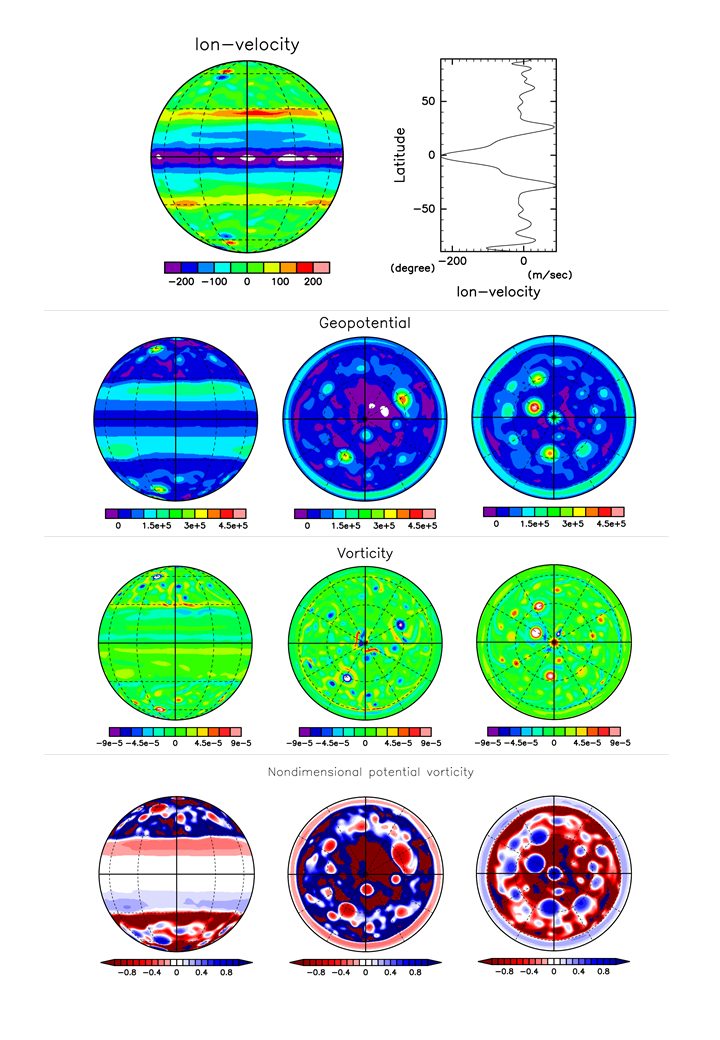
\includegraphics[clip,width=11cm]{./appendix/C/fig_colle/case1/a1_13/1.png}
 \end{center}
 \caption{\footnotesize{ 
}
}
 \label{fig:a1_13_1}
\end{figure}

\begin{figure}[ht]
 \begin{center}
 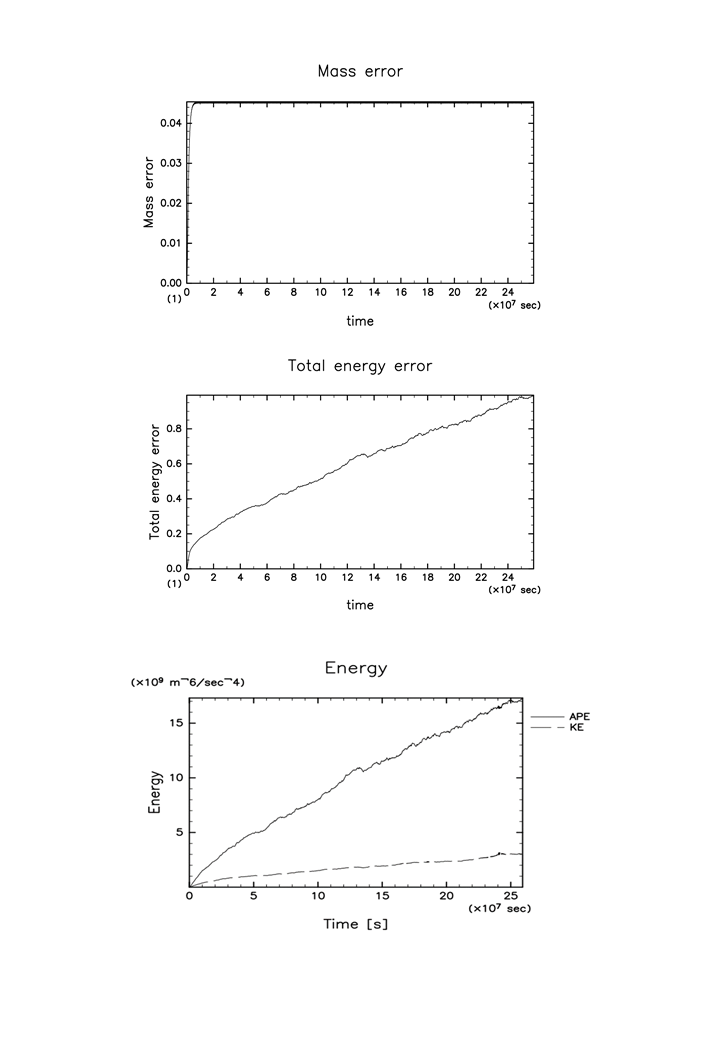
\includegraphics[clip,width=14cm]{./appendix/C/fig_colle/case1/a1_13/2.png}
 \end{center}
 \caption{\footnotesize{
}
}
 \label{fig:a1_13_2}
\end{figure}


%%%%%%%%%%%%%%%%
\def\acknow{謝辞}
\chapter*{\acknow}
\addcontentsline{toc}{chapter}{\acknow}
\label{acknow}
\markright{謝辞}
ddd

\newpage
\renewcommand{\bibname}{参考文献}
\addcontentsline{toc}{chapter}{参考文献}
\bibliographystyle{abbrvnat}
\nocite{*}
\markright{参考文献}
\bibliography{./reference/reference}

\end{document}
